\section{Anlage}
\label{sec:anlage}

\subsection{Segmentplatten}
\label{sec:segments}


\subsection{Gleismaterial}
\label{sec:trackMaterial}


\subsection{Gleiswendel}
\label{sec:trackHelix}

Der H\"ohenunterschied zwischen den Gleisebenen der Bahnho\"ofe Granitz und Schattenwald betr\"agt ca. $16~cm$.
Insbesondere f\"ur die Westausfahrt von Granitz vom schmalen Westsegment aus ist eine einfache Rampe in die $-1$ Ebene aufgrund der hohen Steigung nicht praktikabel.
Somit ergab sich hier erstmalig die Notwendigkeit einer Gleiswendel.

Die Gesamtsituation am Westsegment ist in Abb.~\ref{img:anlage_trackHelix_initialMapSituation} durch den Auszug des Gleisplans zu Beginn der Gleiswendelumsetzung angedeutet.
Das Westsegment hat eine Brei von $45~cm$, in der Abbildung eingerahmt durch den rechten roten Balken, oberen Rasterrand und den angedeuteten roten Strich rechts oben.
Demzufolge ist der Platz f\"ur eine Gleiswendel mit $R1$ am Innen- sowie $R2$ am Au{\ss}engleis bereits nicht ohne weiteres realisierbar.
Als zus\"atzliches Problem an der rechts oberen Ber\"uhrfl\"ache des West- mit dem Zentralsegments kommt der an der Unterseite der Platte angeflanschte Stabilisierungsrahmen hinzu. s.~Abb.~\hl{XX}.
Ohne weitere Ma{\ss}nahmen reicht demzufolge f\"ur die erste Halbwindung nicht allein ein H\"ohenunterschied von ca. $4~cm$ aus, der f\"ur eine einfache Untertunnelung des Plattenbodens selbst n\"otig w\"are.

\begin{figure}[h]
\centering
  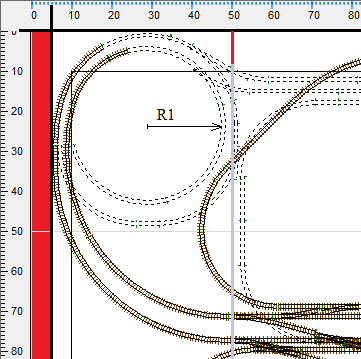
\includegraphics[width=0.35\textwidth]{img/anlage/trackHelix_initialMapSituation.png}
	\caption{Ausgangssituation bei der Planung der Gleiswendel: Westausfahrt von Granitz mit \"Uberf\"uhrung zur Schattenbahnhofsebene}
	\label{img:anlage_trackHelix_initialMapSituation}
\end{figure}

\hl{Lattenrahmen Zentralplatte als Minimap zeigen!}

Angedacht wurde zuerst eine einfache Gleiswendel um ca. $450^\circ$.
Das Innengleis sollte komplett auf $R1$ ausgelegt werden.
F\"ur das Au{\ss}engleis war zumindest in Teilen eine Auslegung mit Flexgleisen geplant.
Die L\"osung der initialen Rahmenunterf\"uhrung wurde zun\"achst aufgeschoben.

Empfehlungen in einschl\"agigen Spur-N Foren nennen Steigungen von $\alpha = \left[ 2 ; 3 \right]^\circ$ als gangbar.
Da dies ganz offensichtlich nicht unter den vorliegenden Randbedingungen eingehalten werden konnte, wurde ein einfacher Testtr\"ager f\"ur die Ermittlung akzeptabler Steigungen erstellt, Abb.~\hl{FIG\_TESTTRAEGER\_STEIGUNG}.
Dieser diente zugleich der Erprobung des h\"aufig angepriesenen Gewindestangenprinzips zur einfachen, flexiblen und gleichzeitig pr\"azisen Justierung der Gleiswendelb\"oden.
Das im Versuchstr\"ager verbaute Gleismaterial war bereits gealtert, um konservativ vorzugehen.
F\"ur die Steigungstests wurde sodann ein Regionalzug verwendet, der als Standard f\"ur das Betriebsszenario von Granitz erachtet wurde.
Die Anzahl der Waggons wurde variiert, um ein Gef\"uhl f\"ur deren Einfluss auf das Verhalten der Lok am Anstieg zu ermitteln.
Insgesamt erschien die Anzahl der Waggons als sekund\"ares Auslegungskriterium.

%25.5 mm

%77 , 77 , 77 mm

%123 mm

Zu den verschiedenen, in Betracht gezogenen Definitionen der Gleiswendel:
\begin{itemize}
	\item Grundlage bildet eine Gleiswendel in Kreis- oder Ovalform.
	\item Bestimmend f\"ur die Auslegung ist das Innengleis mit Verwendung von $R1$ Radien.
	\item Die Radien des Au{\ss}engleises bleiben zun\"achst irrelevant, da gr\"o{\ss}ere Radien bzgl. Steigung unkritischer sind.
	\item Die Fahrwegl\"ange auf einem Viertelkreis ergibt sich somit zu ca. $30~cm$, die eines Halbkreises zu ca. $60~cm$.
	\item Die Ovalisierung der Gleiswendel kann mit beliebigen Standardgr\"o\"{ss}en durchgef\"uhrt werden, im Fall von Arnold N also auf Basis von $5.5~cm$ Geraden, f\"ur alle Steigungsberechnungen konservativ gek\"urzt auf $5~cm$.
\end{itemize}

Mit dem Testtr\"ager ergaben sich Vorergebnisse f\"ur folgende Konfigurationen:
\begin{itemize}
	\item Definition des Versuchstr\"agers:
	\begin{itemize}
		\item Versuchsstrecke Minimum zu Maximum bildet jeweils ein Halboval
		\item Halboval setzt sich zusammen aus $R1 90^\circ$~$\rightarrow$~$22~cm$~\textit{Gerade}~$\rightarrow$~$R1 90^\circ$
		\item Steigung \"uber Gewindestangen justierbar
	\end{itemize}
	\item Standardkonfiguration Testzug: Lok + 3 Doppelstockwagen
	\item H\"ohenunterschied von ca. $2.2~cm$: Gutes Fahrverhalten
	\item H\"ohenunterschied von ca. $5.0~cm$: Noch ausreichendes Fahrverhalten
	\begin{itemize}
		\item Steigung im Versuchstr\"ager: $6.3\%$
		\item Steigung bei m\"oglicher Verl\"angerung der Geraden auf insgesamt 33~cm: $5.6\%$
	\end{itemize}
	\item Die Steigungen \"uberschreiten deutlich die Empfehlungen aus einschl\"agigen Foren.
	\item Es muss ber\"ucksichtigt werden, dass l\"angere Z\"uge und schlechtere Loks ein schlechteres Verhalten an der Steigung aufweisen werden.
	\item[$\Rightarrow$] \textbf{Ein H\"ohenunterschied von $16~cm$ bei einer Windung von $450^\circ$ ist nicht ausreichend.}
\end{itemize}

Aus diesem Grund wurde nun eine doppeletagige Gleiswendel angestrebt.
Tabelle~\ref{tab:anlage_trackHelix_pre_calc_doubleHelix} zeigt hierf\"ur Vorkalkulationen f\"ur resultierende Steigungen.

\begin{table}[h]
	\centering
		\begin{tabular}{lccc}
			H\"ohenunterschied $(cm)$ & Windungen/Etagen $(-)$ & Geradenl\"ange Halboval $(cm)$ & Resultat $\alpha$ $(\%)$ \\
			\hline
			17 & 2 & 20 & 5.3 \\
			17 & 2 & 30 & 4.7 \\
			15 & 2 & 20 & 4.7 \\
			15 & 2 & 25 & 4.5 \\
			15 & 2 & 30 & 4.2 \\
		\end{tabular}
	\caption{Vorrechnungen doppeletagige, ovale Gleiswendel}
	\label{tab:anlage_trackHelix_pre_calc_doubleHelix}
\end{table}








%\begin{figure}[h]
%\centering
	%\begin{subfigure}[b]{0.49\textwidth}
    %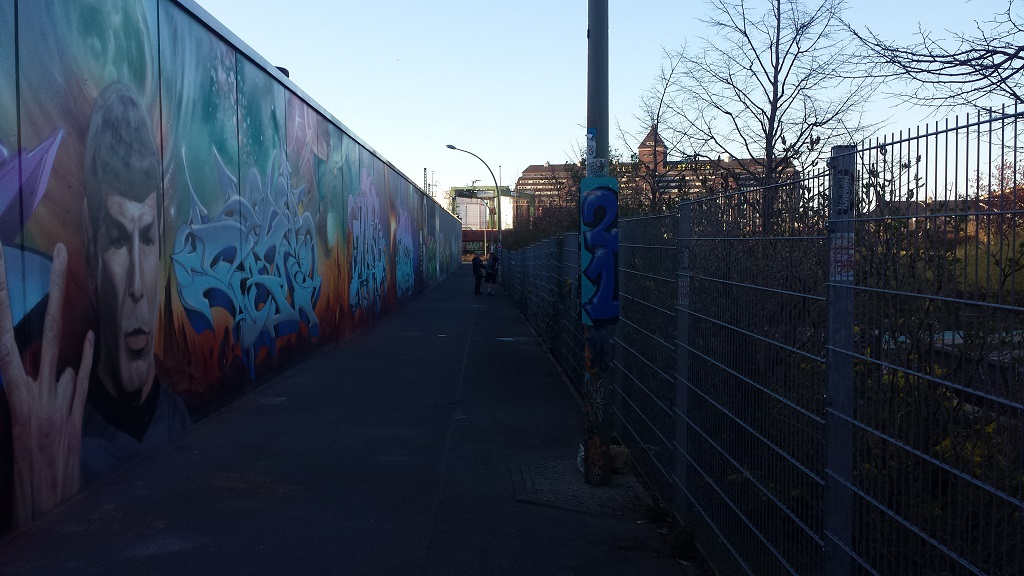
\includegraphics[width=1.0\textwidth]{img/inspiration/westhafen_view_preDurchgang.jpg}
   %\caption{Fu{\ss}g\"angerdurchgang zwischen einem Gro{\ss}handel und dem Stadtgarten am ZK/U, links eine freigegebene Graffitifl\"ache, geradeaus der Westhafen mit vorgelagerter Bahntrasse}
    %\label{img:inspiration_westhafen_view_preDurchgang}
    %\end{subfigure}
	%\begin{subfigure}[b]{0.49\textwidth}
    %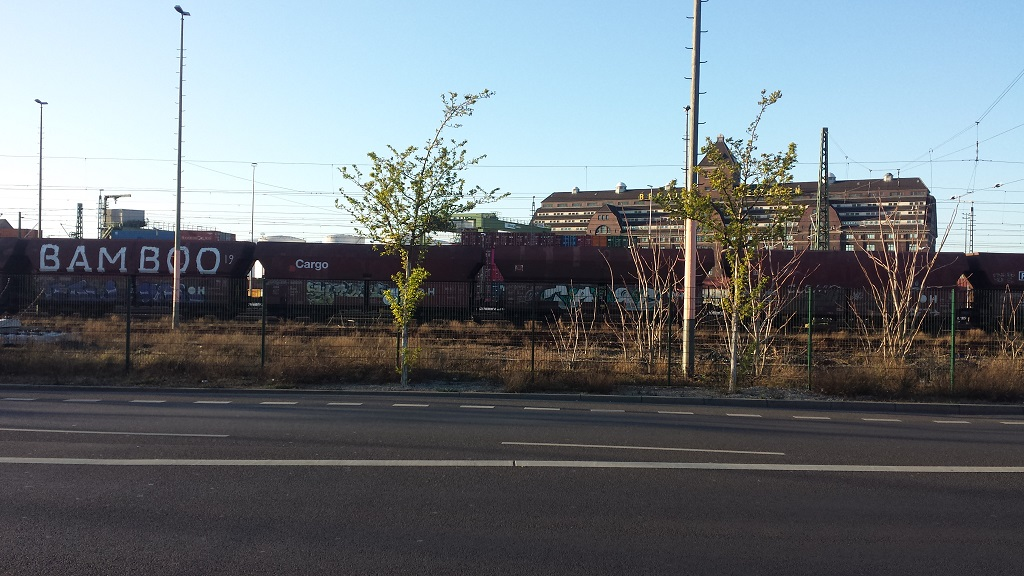
\includegraphics[width=1.0\textwidth]{img/inspiration/westhafen_view_postDurchgang.jpg}
   %\caption{Am Ende des Fu{\ss}g\"angerdurchgangs: typisch abgeranzte Hinterbahnhofshalde mit abgestelltem Lorenzug, irgendwer hat sich daran verewigt, aber niemanden interessiert es}
    %\label{img:inspiration_westhafen_view_postDurchgang}
    %\end{subfigure}
	%\caption{Fu{\ss}g\"angerdurchgang am Stadtgarten des ZK/U Gel\"andes, April 2020 zu einem CoVid-19 Ausgang im eigenen Revier}
	%\label{img:inspiration_westhafen_view_durchgang}
%\end{figure}

